\documentclass[a4paper]{article}
\usepackage[affil-it]{authblk}
\usepackage{amsmath, amssymb}
\usepackage[backend=bibtex,style=numeric]{biblatex}

\usepackage{geometry}
\geometry{margin=1.5cm, vmargin={0pt,1cm}}
\setlength{\topmargin}{-1cm}
\setlength{\paperheight}{29.7cm}
\setlength{\textheight}{25.3cm}

\usepackage{tikz}

\addbibresource{citation.bib}

\begin{document}
% =================================================
\title{Numerical Analysis homework 3 }

\author{Zhang Zihao 3230101685
  \thanks{Electronic address: \texttt{3230101685@zju.edu.cn}}}
\affil{(Information and Computing Science 1), Zhejiang University }


\date{Due time: \today}

\maketitle

\begin{abstract}
    My homework for numerical analysis.     
\end{abstract}

% ============================================
\begin{document}

\section*{Problem I: Cubic Spline Analysis}
\subsection*{Problem Statement}
Consider \( s \in S^2_3 \) on \([0, 2]\):

\[
s(x) = 
\begin{cases} 
p(x) & \text{if } x \in [0, 1], \\
(2 - x)^3 & \text{if } x \in [1, 2].
\end{cases}
\]

Determine \( p \in \mathbb{P}_3 \) such that \( s(0) = 0 \). Is \( s(x) \) a natural cubic spline?

\subsection*{Solution}

\paragraph*{Polynomial form and boundary condition:}
Let \( p(x) = ax^3 + bx^2 + cx + d \). Using the boundary condition:
\[
s(0) = p(0) = d = 0 \quad \Rightarrow \quad d = 0
\]
Thus, \( p(x) = ax^3 + bx^2 + cx \).

\paragraph*{Continuity conditions at \( x = 1 \):}
Let \( q(x) = (2 - x)^3 \). We require:

\begin{itemize}
\item \textbf{Function value continuity:}
\[
p(1) = q(1) \Rightarrow a + b + c = (2-1)^3 = 1 \quad \text{(1)}
\]

\item \textbf{First derivative continuity:}
\[
p'(x) = 3ax^2 + 2bx + c, \quad q'(x) = -3(2-x)^2
\]
\[
p'(1) = q'(1) \Rightarrow 3a + 2b + c = -3(2-1)^2 = -3 \quad \text{(2)}
\]

\item \textbf{Second derivative continuity:}
\[
p''(x) = 6ax + 2b, \quad q''(x) = 6(2-x)
\]
\[
p''(1) = q''(1) \Rightarrow 6a + 2b = 6(2-1) = 6 \quad \text{(3)}
\end{itemize}

\paragraph*{Solving the system:}
We solve the system of equations:

From equation (3): \( 6a + 2b = 6 \Rightarrow 3a + b = 3 \) \quad \text{(3a)}

Subtract equation (1) from equation (2):
\[
(3a + 2b + c) - (a + b + c) = -3 - 1 \Rightarrow 2a + b = -4 \quad \text{(4)}
\]

Subtract equation (4) from equation (3a):
\[
(3a + b) - (2a + b) = 3 - (-4) \Rightarrow a = 7
\]

Substitute \( a = 7 \) into equation (3a):
\[
3(7) + b = 3 \Rightarrow 21 + b = 3 \Rightarrow b = -18
\]

Substitute \( a = 7, b = -18 \) into equation (1):
\[
7 - 18 + c = 1 \Rightarrow -11 + c = 1 \Rightarrow c = 12
\]

Compute:
\[
s''(0) = p''(0) = 6a(0) + 2b = 2(-18) = -36 \neq 0
\]
\[
s''(2) = q''(2) = 6(2-2) = 0
\]

Since \( s''(0) \neq 0 \), the spline is not natural.

\subsection*{Final Answers:}
\begin{enumerate}
\item \( p(x) = 7x^3 - 18x^2 + 12x \)
\item \( s(x) \) is \textbf{not} a natural cubic spline because \( s''(0) = -36 \neq 0 \)
\end{enumerate}



\section*{Problem II: Quadratic Spline Interpolation}
\subsection*{Problem Statement}
Given \( f_i = f(x_i) \) of some scalar function at points  
\( a = x_1 < x_2 < \cdots < x_n = b \), we consider interpolating  
\( f \) on \([a, b]\) with a quadratic spline \( s \in \mathbb{S}_2^1 \).  

\begin{enumerate}
\item[(a)] Why is an additional condition needed to determine \( s \) uniquely?  

\item[(b)] Define \( m_i = s'(x_i) \) and \( p_i = s|_{[x_i,x_{i+1}]} \).  
Determine \( p_i \) in terms of \( f_i, f_{i+1} \), and \( m_i \) for  
\( i = 1, 2, \ldots, n-1 \).  

\item[(c)] Suppose \( m_1 = f'(a) \) is given. Show how  
\( m_2, m_3, \ldots, m_{n-1} \) can be computed.
\end{enumerate}

\subsection*{Solution}

\paragraph*{(a) Uniqueness and additional condition:}
A quadratic spline \( s \in \mathbb{S}_2^1 \) on \( n \) nodes consists of \( n-1 \) quadratic polynomial pieces. Let's count the degrees of freedom and constraints precisely.

\textbf{Degrees of freedom:}
\begin{itemize}
\item Each quadratic polynomial piece has 3 parameters.
\item Total parameters: \( 3(n-1) = 3n - 3 \).
\end{itemize}

\textbf{Constraints:}
\begin{itemize}
\item \textbf{Interpolation conditions:}
  \begin{itemize}
  \item At the first node \( x_1 \): 1 condition (\( s_1(x_1) = f_1 \))
  \item At the last node \( x_n \): 1 condition (\( s_{n-1}(x_n) = f_n \))
  \item At each interior node \( x_i \) (\( i = 2, \ldots, n-1 \)): 2 conditions \\
        (\( s_{i-1}(x_i) = f_i \) and \( s_i(x_i) = f_i \))
  \item Total interpolation conditions: \( 1 + 1 + 2(n-2) = 2n - 2 \)
  \end{itemize}

\item \textbf{First derivative continuity conditions (C¹):}
  \begin{itemize}
  \item At each interior node \( x_i \) (\( i = 2, \ldots, n-1 \)): 1 condition \\
        (\( s'_{i-1}(x_i) = s'_i(x_i) \))
  \item Total C¹ conditions: \( n - 2 \)
  \end{itemize}
\end{itemize}

\textbf{Total constraints:} \( (2n - 2) + (n - 2) = 3n - 4 \)

Since we have \( 3n - 3 \) degrees of freedom but only \( 3n - 4 \) constraints, we are short by \textbf{one} condition to determine the spline uniquely.

\paragraph*{(b) Expression for the quadratic polynomial piece:}

Using the given conditions:
\begin{itemize}
    \item \( p_i(x_i) = f_i \)
    \item \( p_i(x_{i+1}) = f_{i+1} \)
    \item \( p_i'(x_i) = m_i \)
\end{itemize}

Let \( p_i(x) = a_i(x - x_i)^2 + b_i(x - x_i) + c_i \). From the conditions:

\begin{itemize}
    \item \( p_i(x_i) = c_i = f_i \)
    \item \( p_i'(x_i) = b_i = m_i \)
    \item \( p_i(x_{i+1}) = a_i h_i^2 + m_i h_i + f_i = f_{i+1} \Rightarrow a_i = \dfrac{f_{i+1} - f_i - m_i h_i}{h_i^2} \)
\end{itemize}

Therefore, the quadratic polynomial is:
\[
p_i(x) = \frac{f_{i+1} - f_i - m_i h_i}{h_i^2}(x - x_i)^2 + m_i(x - x_i) + f_i
\]
where \( h_i = x_{i+1} - x_i \).

\paragraph*{(c) Recursive computation of \( m_i \):}
Using the expression for \( p_i(x) \) from part (b):
\[
p_i(x) = \frac{f_{i+1} - f_i - m_i h_i}{h_i^2}(x - x_i)^2 + m_i(x - x_i) + f_i
\]

Differentiate to find the derivative:
\[
p_i'(x) = \frac{2(f_{i+1} - f_i - m_i h_i)}{h_i^2}(x - x_i) + m_i
\]

Now evaluate at the right endpoint \( x = x_{i+1} \):
\[
p_i'(x_{i+1}) = \frac{2(f_{i+1} - f_i - m_i h_i)}{h_i^2} \cdot h_i + m_i = \frac{2(f_{i+1} - f_i - m_i h_i)}{h_i} + m_i
\]

Simplify:
\[
p_i'(x_{i+1}) = \frac{2(f_{i+1} - f_i)}{h_i} - 2m_i + m_i = \frac{2(f_{i+1} - f_i)}{h_i} - m_i
\]

By the continuity of the first derivative (\( C^1 \) continuity) at interior nodes, we have:
\[
p_i'(x_{i+1}) = p_{i+1}'(x_{i+1}) = m_{i+1}
\]

Therefore, we obtain the recurrence relation:
\[
m_{i+1} = \frac{2(f_{i+1} - f_i)}{h_i} - m_i, \quad \text{for } i = 1, 2, \ldots, n-1
\]

Given \( m_1 = f'(a) \), we can compute sequentially:
\[
\begin{aligned}
m_2 &= \frac{2(f_2 - f_1)}{h_1} - m_1 \\
m_3 &= \frac{2(f_3 - f_2)}{h_2} - m_2 \\
&\vdots \\
m_{n-1} &= \frac{2(f_{n-1} - f_{n-2})}{h_{n-2}} - m_{n-2}
\end{aligned}
\]

This recurrence allows us to compute all the derivatives \( m_2, m_3, \ldots, m_n \) starting from the given initial condition \( m_1 \).




\section*{Problem III: Natural Cubic Spline Construction}
\subsection*{Problem Statement}
Let \( s_1(x) = 1 + c(x+1)^3 \) where \( x \in [-1,0] \) and \( c \in \mathbb{R} \).  
Determine \( s_2(x) \) on \([0,1]\) such that  

\[
s(x) =
\begin{cases} 
s_1(x) & \text{if } x \in [-1,0], \\
s_2(x) & \text{if } x \in [0,1]
\end{cases}
\]

is a natural cubic spline on \([-1,1]\) with knots \(-1,0,1\).  
How must \( c \) be chosen if one wants \( s(1) = -1 \)?

\subsection*{Solution}

\paragraph*{Step 1: General form of \( s_2(x) \)}
Since \( s \) is a cubic spline, \( s_2(x) \) must be a cubic polynomial on \([0,1]\). Let
\[
s_2(x) = A + Bx + Cx^2 + Dx^3.
\]

\paragraph*{Step 2: Continuity conditions at \( x = 0 \)}
We require \( C^2 \) continuity at the knot \( x = 0 \).

Function value continuity:
\[
s_1(0) = s_2(0) \Rightarrow 1 + c(0+1)^3 = A \Rightarrow 1 + c = A. \quad \text{(1)}
\]

First derivative continuity:
\[
s_1'(x) = 3c(x+1)^2, \quad s_2'(x) = B + 2Cx + 3Dx^2.
\]
\[
s_1'(0) = s_2'(0) \Rightarrow 3c(1)^2 = B \Rightarrow 3c = B. \quad \text{(2)}
\]

Second derivative continuity:
\[
s_1''(x) = 6c(x+1), \quad s_2''(x) = 2C + 6Dx.
\]
\[
s_1''(0) = s_2''(0) \Rightarrow 6c(1) = 2C \Rightarrow 6c = 2C \Rightarrow C = 3c. \quad \text{(3)}
\end{itemize}




\paragraph*{Step 3: Natural boundary conditions}
A natural cubic spline requires zero second derivatives at the endpoints.

\begin{itemize}
\item At \( x = -1 \):
\[
s_1''(-1) = 6c(-1+1) = 0 
\]

\item At \( x = 1 \):
\[
s_2''(1) = 2C + 6D(1) = 0 \Rightarrow 2C + 6D = 0. \quad \text{(4)}
\]
\end{itemize}

\paragraph*{Step 4: Solve for coefficients}
From (3): \( C = 3c \).  
Substitute into (4):
\[
2(3c) + 6D = 0 \Rightarrow 6c + 6D = 0 \Rightarrow D = -c.
\]

So far we have:
\[
A = 1 + c, \quad B = 3c, \quad C = 3c, \quad D = -c.
\]

Thus:
\[
s_2(x) = (1 + c) + 3c x + 3c x^2 - c x^3.
\]

\paragraph*{Step 5: Additional condition \( s(1) = -1 \)}
\[
s_2(1) = (1 + c) + 3c(1) + 3c(1)^2 - c(1)^3 = 1 + c + 3c + 3c - c = 1 + 6c.
\]
Set \( s_2(1) = -1 \):
\[
1 + 6c = -1 \Rightarrow 6c = -2 \Rightarrow c = -\frac{1}{3}.
\]

\paragraph*{Step 6: Final expression for \( s_2(x) \)}
Substitute \( c = -\frac{1}{3} \) into \( s_2(x) \):
\[
s_2(x) = \left(1 - \frac{1}{3}\right) + 3\left(-\frac{1}{3}\right)x + 3\left(-\frac{1}{3}\right)x^2 - \left(-\frac{1}{3}\right)x^3
\]
\[
s_2(x) = \frac{2}{3} - x - x^2 + \frac{1}{3}x^3.
\]

\subsection*{Final Answers:}
\begin{enumerate}
\item The cubic polynomial on \([0,1]\) is:
\[
s_2(x) = (1 + c) + 3c x + 3c x^2 - c x^3
\]

\item For \( s(1) = -1 \), we must choose:
\[
c = -\frac{1}{3}
\]
and then
\[
s_2(x) = \frac{2}{3} - x - x^2 + \frac{1}{3}x^3
\]
\end{enumerate}


\section*{Problem IV: Natural Cubic Spline and Bending Energy}
\subsection*{Problem Statement}
Consider \( f(x) = \cos\left(\frac{\pi}{2}x\right) \) with \( x \in [-1, 1] \).

\begin{enumerate}
\item[(a)] Determine the natural cubic spline interpolant to \( f \) on knots \(-1, 0, 1\).

\item[(b)] As discussed in the class, natural cubic splines have the minimal total bending energy. Verify this by taking \( g(x) \) to be (i) the quadratic polynomial that interpolates \( f \) at \(-1, 0, 1\), and (ii) \( f(x) \).
\end{enumerate}

\subsection*{Solution}

\paragraph*{(a) Natural cubic spline interpolant}

Let the cubic spline be defined as:
\[
s(x) = 
\begin{cases} 
s_1(x) = a_1 + b_1(x+1) + c_1(x+1)^2 + d_1(x+1)^3, & x \in [-1, 0] \\
s_2(x) = a_2 + b_2x + c_2x^2 + d_2x^3, & x \in [0, 1]
\end{cases}
\]

First, compute the function values at the knots:
\[
f(-1) = \cos\left(-\frac{\pi}{2}\right) = 0, \quad f(0) = \cos(0) = 1, \quad f(1) = \cos\left(\frac{\pi}{2}\right) = 0
\]

\subparagraph*{Interpolation conditions:}
\begin{align*}
s_1(-1) &= a_1 = 0 \quad \text{(1)} \\
s_1(0) &= a_1 + b_1 + c_1 + d_1 = 1 \quad \text{(2)} \\
s_2(0) &= a_2 = 1 \quad \text{(3)} \\
s_2(1) &= a_2 + b_2 + c_2 + d_2 = 0 \quad \text{(4)}
\end{align*}

\subparagraph*{Continuity of first derivative at \( x = 0 \):}
\begin{align*}
s_1'(x) &= b_1 + 2c_1(x+1) + 3d_1(x+1)^2 \\
s_2'(x) &= b_2 + 2c_2x + 3d_2x^2 \\
s_1'(0) &= b_1 + 2c_1 + 3d_1 = s_2'(0) = b_2 \quad \text{(5)}
\end{align*}

\subparagraph*{Continuity of second derivative at \( x = 0 \):}
\begin{align*}
s_1''(x) &= 2c_1 + 6d_1(x+1) \\
s_2''(x) &= 2c_2 + 6d_2x \\
s_1''(0) &= 2c_1 + 6d_1 = s_2''(0) = 2c_2 \quad \text{(6)}
\end{align*}

\subparagraph*{Natural boundary conditions:}
\begin{align*}
s_1''(-1) &= 2c_1 = 0 \Rightarrow c_1 = 0 \quad \text{(7)} \\
s_2''(1) &= 2c_2 + 6d_2 = 0 \quad \text{(8)}
\end{align*}

\subparagraph*{Solve the system:}
From (7): \( c_1 = 0 \)

From (1): \( a_1 = 0 \)

From (3): \( a_2 = 1 \)

From (2): \( b_1 + d_1 = 1 \quad \text{(2a)} \)

From (6): \( 6d_1 = 2c_2 \Rightarrow c_2 = 3d_1 \quad \text{(6a)} \)

From (8): \( 2c_2 + 6d_2 = 0 \Rightarrow 6d_1 + 6d_2 = 0 \Rightarrow d_2 = -d_1 \quad \text{(8a)} \)

From (4): \( 1 + b_2 + c_2 + d_2 = 0 \Rightarrow b_2 + c_2 + d_2 = -1 \quad \text{(4a)} \)

Substitute (6a) and (8a) into (4a):
\[
b_2 + 3d_1 - d_1 = -1 \Rightarrow b_2 + 2d_1 = -1 \quad \text{(4b)}
\]

From (5): \( b_2 = b_1 + 3d_1 \quad \text{(5a)} \)

Substitute (5a) into (4b):
\[
b_1 + 3d_1 + 2d_1 = -1 \Rightarrow b_1 + 5d_1 = -1 \quad \text{(4c)}
\]

Now solve the system of (2a) and (4c):
\[
\begin{cases}
b_1 + d_1 = 1 \\
b_1 + 5d_1 = -1
\end{cases}
\]

Subtract the first equation from the second:
\[
4d_1 = -2 \Rightarrow d_1 = -\frac{1}{2}
\]

Then:
\[
b_1 = 1 - d_1 = 1 + \frac{1}{2} = \frac{3}{2}
\]

From (5a): \( b_2 = b_1 + 3d_1 = \frac{3}{2} - \frac{3}{2} = 0 \)

From (6a): \( c_2 = 3d_1 = -\frac{3}{2} \)

From (8a): \( d_2 = -d_1 = \frac{1}{2} \)

\subparagraph*{Final spline functions:}
\[
s_1(x) = \frac{3}{2}(x+1) - \frac{1}{2}(x+1)^3, \quad x \in [-1, 0]
\]
\[
s_2(x) = 1 - \frac{3}{2}x^2 + \frac{1}{2}x^3, \quad x \in [0, 1]
\]

\paragraph*{(b) Bending energy comparison}

The bending energy is defined as:
\[
E[g] = \int_{-1}^1 [g''(x)]^2 dx
\]

\subparagraph*{(i) Quadratic polynomial interpolant:}
Let \( g(x) = Ax^2 + Bx + C \). Using interpolation conditions:
\begin{align*}
g(-1) &= A - B + C = 0 \\
g(0) &= C = 1 \\
g(1) &= A + B + C = 0
\end{align*}

Solving: \( C = 1 \), and from the first and third equations:
\[
A - B = -1, \quad A + B = -1
\]
Adding: \( 2A = -2 \Rightarrow A = -1 \), then \( B = 0 \).

So \( g(x) = -x^2 + 1 \), and \( g''(x) = -2 \).

Bending energy:
\[
E[g] = \int_{-1}^1 (-2)^2 dx = 4 \times 2 = 8
\]

\subparagraph*{(ii) Original function \( f(x) \):}
\[
f(x) = \cos\left(\frac{\pi}{2}x\right), \quad f'(x) = -\frac{\pi}{2}\sin\left(\frac{\pi}{2}x\right), \quad f''(x) = -\frac{\pi^2}{4}\cos\left(\frac{\pi}{2}x\right)
\]

Bending energy:
\[
E[f] = \int_{-1}^1 \left[-\frac{\pi^2}{4}\cos\left(\frac{\pi}{2}x\right)\right]^2 dx = \frac{\pi^4}{16} \int_{-1}^1 \cos^2\left(\frac{\pi}{2}x\right) dx
\]

Using the identity \( \cos^2\theta = \frac{1 + \cos 2\theta}{2} \):
\[
E[f] = \frac{\pi^4}{16} \int_{-1}^1 \frac{1 + \cos(\pi x)}{2} dx = \frac{\pi^4}{32} \left[ \int_{-1}^1 1 dx + \int_{-1}^1 \cos(\pi x) dx \right]
\]

Since \( \int_{-1}^1 \cos(\pi x) dx = \left[\frac{\sin(\pi x)}{\pi}\right]_{-1}^1 = 0 \), we have:
\[
E[f] = \frac{\pi^4}{32} \times 2 = \frac{\pi^4}{16} \approx \frac{97.4091}{16} \approx 6.088
\]

\subparagraph*{(iii) Natural cubic spline \( s(x) \):}
Compute second derivatives:
\[
s_1''(x) = -3(x+1), \quad s_2''(x) = -3 + 3x
\]

Bending energy:
\[
E[s] = \int_{-1}^0 [-3(x+1)]^2 dx + \int_0^1 [-3 + 3x]^2 dx
\]
\[
= 9\int_{-1}^0 (x+1)^2 dx + 9\int_0^1 (1 - x)^2 dx
\]
\[
= 9\left[\frac{(x+1)^3}{3}\right]_{-1}^0 + 9\left[-\frac{(1-x)^3}{3}\right]_0^1
\]
\[
= 3[(1)^3 - (0)^3] + 3[0 - (-1)^3] = 3(1) + 3(1) = 6
\]

\subparagraph*{Comparison:}
\[
E[s] = 6 < E[f] \approx 6.088 < E[g] = 8
\]

This verifies that the natural cubic spline has the minimal bending energy.


\section*{Problem V: The Quadratic B-spline \( B_i^2(x) \)}

\subsection*{Problem Statement}
\begin{enumerate}
\item[(a)] Derive the same explicit expression of \( B_i^2(x) \) as that in the notes from the recursive definition of B-splines and the hat function.

\item[(b)] Verify that \( \frac{d}{dx} B_i^2(x) \) is continuous at \( t_i \) and \( t_{i+1} \).

\item[(c)] Show that only one \( x^* \in (t_{i-1}, t_{i+2}) \) satisfies \( \frac{d}{dx} B_i^2(x^*) = 0 \). Express \( x^* \) in terms of the knots within the interval of support.

\item[(d)] Consequently, show \( B_i^2(x) \in [0, 1) \).

\item[(e)] Plot \( B_i^2(x) \) for \( t_i = i \).
\end{enumerate}

\subsection*{Solution}

\paragraph*{(a) Derivation of explicit expression}

Using the recursive definition:
\[
B_{i}^{n+1}(x) = \frac{x - t_{i-1}}{t_{i+n} - t_{i-1}} B_{i}^{n}(x) + \frac{t_{i+n+1} - x}{t_{i+n+1} - t_{i}} B_{i+1}^{n}(x)
\]
with base case:
\[
B_{i}^{0}(x) = 
\begin{cases} 
1 & \text{if } x \in (t_{i-1}, t_{i}) \\
0 & \text{otherwise}
\end{cases}
\]

For quadratic B-splines (\( n = 2 \)), we have:
\[
B_i^2(x) = \frac{x - t_{i-1}}{t_{i+1} - t_{i-1}} B_i^1(x) + \frac{t_{i+2} - x}{t_{i+2} - t_i} B_{i+1}^1(x)
\]

First, compute the linear B-splines:
\[
B_i^1(x) = \frac{x - t_{i-1}}{t_i - t_{i-1}} B_i^0(x) + \frac{t_{i+1} - x}{t_{i+1} - t_i} B_{i+1}^0(x)
\]
\[
B_{i+1}^1(x) = \frac{x - t_i}{t_{i+1} - t_i} B_{i+1}^0(x) + \frac{t_{i+2} - x}{t_{i+2} - t_{i+1}} B_{i+2}^0(x)
\]

The support of \( B_i^2(x) \) is \( (t_{i-1}, t_{i+2}) \). We analyze piece by piece:

\subparagraph*{Interval 1: \( (t_{i-1}, t_i) \)}
On this interval: \( B_i^0(x) = 1 \), \( B_{i+1}^0(x) = 0 \), \( B_{i+2}^0(x) = 0 \)

Thus:
\[
B_i^1(x) = \frac{x - t_{i-1}}{t_i - t_{i-1}}, \quad B_{i+1}^1(x) = 0
\]
\[
B_i^2(x) = \frac{x - t_{i-1}}{t_{i+1} - t_{i-1}} \cdot \frac{x - t_{i-1}}{t_i - t_{i-1}} = \frac{(x - t_{i-1})^2}{(t_{i+1} - t_{i-1})(t_i - t_{i-1})}
\]

\subparagraph*{Interval 2: \( (t_i, t_{i+1}) \)}
On this interval: \( B_i^0(x) = 0 \), \( B_{i+1}^0(x) = 1 \), \( B_{i+2}^0(x) = 0 \)

Thus:
\[
B_i^1(x) = \frac{t_{i+1} - x}{t_{i+1} - t_i}, \quad B_{i+1}^1(x) = \frac{x - t_i}{t_{i+1} - t_i}
\]
\[
B_i^2(x) = \frac{x - t_{i-1}}{t_{i+1} - t_{i-1}} \cdot \frac{t_{i+1} - x}{t_{i+1} - t_i} + \frac{t_{i+2} - x}{t_{i+2} - t_i} \cdot \frac{x - t_i}{t_{i+1} - t_i}
\]

\subparagraph*{Interval 3: \( (t_{i+1}, t_{i+2}) \)}
On this interval: \( B_i^0(x) = 0 \), \( B_{i+1}^0(x) = 0 \), \( B_{i+2}^0(x) = 1 \)

Thus:
\[
B_i^1(x) = 0, \quad B_{i+1}^1(x) = \frac{t_{i+2} - x}{t_{i+2} - t_{i+1}}
\]
\[
B_i^2(x) = \frac{t_{i+2} - x}{t_{i+2} - t_i} \cdot \frac{t_{i+2} - x}{t_{i+2} - t_{i+1}} = \frac{(t_{i+2} - x)^2}{(t_{i+2} - t_i)(t_{i+2} - t_{i+1})}
\]

This matches the expression given in Example 3.25.

\paragraph*{(b) Continuity of derivative}

We verify that \( \frac{d}{dx} B_i^2(x) \) is continuous at both \( t_i \) and \( t_{i+1} \).

\subparagraph*{At \( x = t_i \):}

From Interval 1 \( (t_{i-1}, t_i) \):
\[
B_i^2(x) = \frac{(x - t_{i-1})^2}{(t_{i+1} - t_{i-1})(t_i - t_{i-1})}
\]
\[
\frac{d}{dx}B_i^2(x) = \frac{2(x - t_{i-1})}{(t_{i+1} - t_{i-1})(t_i - t_{i-1})}
\]
At \( x = t_i^- \):
\[
\frac{d}{dx}B_i^2(t_i^-) = \frac{2(t_i - t_{i-1})}{(t_{i+1} - t_{i-1})(t_i - t_{i-1})} = \frac{2}{t_{i+1} - t_{i-1}}
\]

From Interval 2 \( (t_i, t_{i+1}) \):
\[
B_i^2(x) = \frac{x - t_{i-1}}{t_{i+1} - t_{i-1}} \cdot \frac{t_{i+1} - x}{t_{i+1} - t_i} + \frac{t_{i+2} - x}{t_{i+2} - t_i} \cdot \frac{x - t_i}{t_{i+1} - t_i}
\]

Differentiate term by term:
\begin{align*}
\frac{d}{dx}B_i^2(x) =& \frac{1}{t_{i+1} - t_{i-1}} \cdot \frac{t_{i+1} - x}{t_{i+1} - t_i} + \frac{x - t_{i-1}}{t_{i+1} - t_{i-1}} \cdot \frac{-1}{t_{i+1} - t_i} \\
&+ \frac{-1}{t_{i+2} - t_i} \cdot \frac{x - t_i}{t_{i+1} - t_i} + \frac{t_{i+2} - x}{t_{i+2} - t_i} \cdot \frac{1}{t_{i+1} - t_i}
\end{align*}

At \( x = t_i^+ \):
\begin{align*}
\frac{d}{dx}B_i^2(t_i^+) =& \frac{1}{t_{i+1} - t_{i-1}} \cdot \frac{t_{i+1} - t_i}{t_{i+1} - t_i} + \frac{t_i - t_{i-1}}{t_{i+1} - t_{i-1}} \cdot \frac{-1}{t_{i+1} - t_i} \\
&+ \frac{-1}{t_{i+2} - t_i} \cdot \frac{t_i - t_i}{t_{i+1} - t_i} + \frac{t_{i+2} - t_i}{t_{i+2} - t_i} \cdot \frac{1}{t_{i+1} - t_i}
\end{align*}

Simplify:
\begin{align*}
\frac{d}{dx}B_i^2(t_i^+) =& \frac{1}{t_{i+1} - t_{i-1}} - \frac{t_i - t_{i-1}}{(t_{i+1} - t_{i-1})(t_{i+1} - t_i)} + 0 + \frac{1}{t_{i+1} - t_i} \\
=& \frac{1}{t_{i+1} - t_{i-1}} + \frac{1}{t_{i+1} - t_i} - \frac{t_i - t_{i-1}}{(t_{i+1} - t_{i-1})(t_{i+1} - t_i)}
\end{align*}

Combine over common denominator \( (t_{i+1} - t_{i-1})(t_{i+1} - t_i) \):
\begin{align*}
\frac{d}{dx}B_i^2(t_i^+) =& \frac{t_{i+1} - t_i + t_{i+1} - t_{i-1} - (t_i - t_{i-1})}{(t_{i+1} - t_{i-1})(t_{i+1} - t_i)} \\
=& \frac{t_{i+1} - t_i + t_{i+1} - t_{i-1} - t_i + t_{i-1}}{(t_{i+1} - t_{i-1})(t_{i+1} - t_i)} \\
=& \frac{2(t_{i+1} - t_i)}{(t_{i+1} - t_{i-1})(t_{i+1} - t_i)} = \frac{2}{t_{i+1} - t_{i-1}}
\end{align*}

Thus: \( \frac{d}{dx}B_i^2(t_i^-) = \frac{2}{t_{i+1} - t_{i-1}} = \frac{d}{dx}B_i^2(t_i^+) \)

\subparagraph*{At \( x = t_{i+1} \):}

From Interval 2 \( (t_i, t_{i+1}) \):
At \( x = t_{i+1}^- \):
\begin{align*}
\frac{d}{dx}B_i^2(t_{i+1}^-) =& \frac{t_{i+1} + t_{i-1} - 2t_{i+1}}{(t_{i+1} - t_{i-1})(t_{i+1} - t_i)} + \frac{t_{i+2} + t_i - 2t_{i+1}}{(t_{i+2} - t_i)(t_{i+1} - t_i)} \\
=& \frac{t_{i-1} - t_{i+1}}{(t_{i+1} - t_{i-1})(t_{i+1} - t_i)} + \frac{t_{i+2} + t_i - 2t_{i+1}}{(t_{i+2} - t_i)(t_{i+1} - t_i)} \\
=& \frac{-(t_{i+1} - t_{i-1})}{(t_{i+1} - t_{i-1})(t_{i+1} - t_i)} + \frac{t_{i+2} + t_i - 2t_{i+1}}{(t_{i+2} - t_i)(t_{i+1} - t_i)} \\
=& \frac{-1}{t_{i+1} - t_i} + \frac{t_{i+2} + t_i - 2t_{i+1}}{(t_{i+2} - t_i)(t_{i+1} - t_i)}
\end{align*}

From Interval 3 \( (t_{i+1}, t_{i+2}) \):
\[
B_i^2(x) = \frac{(t_{i+2} - x)^2}{(t_{i+2} - t_i)(t_{i+2} - t_{i+1})}
\]
\[
\frac{d}{dx}B_i^2(x) = \frac{-2(t_{i+2} - x)}{(t_{i+2} - t_i)(t_{i+2} - t_{i+1})}
\]
At \( x = t_{i+1}^+ \):
\[
\frac{d}{dx}B_i^2(t_{i+1}^+) = \frac{-2(t_{i+2} - t_{i+1})}{(t_{i+2} - t_i)(t_{i+2} - t_{i+1})} = \frac{-2}{t_{i+2} - t_i}
\]

Now show equality:
\begin{align*}
\frac{d}{dx}B_i^2(t_{i+1}^-) =& \frac{-1}{t_{i+1} - t_i} + \frac{t_{i+2} + t_i - 2t_{i+1}}{(t_{i+2} - t_i)(t_{i+1} - t_i)} \\
=& \frac{-(t_{i+2} - t_i) + (t_{i+2} + t_i - 2t_{i+1})}{(t_{i+2} - t_i)(t_{i+1} - t_i)} \\
=& \frac{-t_{i+2} + t_i + t_{i+2} + t_i - 2t_{i+1}}{(t_{i+2} - t_i)(t_{i+1} - t_i)} \\
=& \frac{2t_i - 2t_{i+1}}{(t_{i+2} - t_i)(t_{i+1} - t_i)} = \frac{-2(t_{i+1} - t_i)}{(t_{i+2} - t_i)(t_{i+1} - t_i)} = \frac{-2}{t_{i+2} - t_i}
\end{align*}

Thus: \( \frac{d}{dx}B_i^2(t_{i+1}^-) = \frac{-2}{t_{i+2} - t_i} = \frac{d}{dx}B_i^2(t_{i+1}^+) \)

\paragraph*{(c) Unique critical point}

We analyze the derivative on each interval to show there exists exactly one critical point.

\subparagraph*{Interval 1: \( (t_{i-1}, t_i) \)}
\[
\frac{d}{dx}B_i^2(x) = \frac{2(x - t_{i-1})}{(t_{i+1} - t_{i-1})(t_i - t_{i-1})}
\]
Since \( x - t_{i-1} > 0 \) and all denominators are positive, \( \frac{d}{dx}B_i^2(x) > 0 \) for all \( x \in (t_{i-1}, t_i) \). No critical points in this interval.

\subparagraph*{Interval 3: \( (t_{i+1}, t_{i+2}) \)}
\[
\frac{d}{dx}B_i^2(x) = \frac{-2(t_{i+2} - x)}{(t_{i+2} - t_i)(t_{i+2} - t_{i+1})}
\]
Since \( t_{i+2} - x > 0 \) and all denominators are positive, \( \frac{d}{dx}B_i^2(x) < 0 \) for all \( x \in (t_{i+1}, t_{i+2}) \). No critical points in this interval.

\subparagraph*{Interval 2: \( (t_i, t_{i+1}) \)}
The derivative is:
\[
\frac{d}{dx}B_i^2(x) = \frac{t_{i+1} + t_{i-1} - 2x}{(t_{i+1} - t_{i-1})(t_{i+1} - t_i)} + \frac{t_{i+2} + t_i - 2x}{(t_{i+2} - t_i)(t_{i+1} - t_i)}
\]

Set \( \frac{d}{dx}B_i^2(x) = 0 \):
\[
\frac{t_{i+1} + t_{i-1} - 2x}{(t_{i+1} - t_{i-1})(t_{i+1} - t_i)} + \frac{t_{i+2} + t_i - 2x}{(t_{i+2} - t_i)(t_{i+1} - t_i)} = 0
\]

Multiply through by \( (t_{i+1} - t_i) \):
\[
\frac{t_{i+1} + t_{i-1} - 2x}{t_{i+1} - t_{i-1}} + \frac{t_{i+2} + t_i - 2x}{t_{i+2} - t_i} = 0
\]

Let \( A = \frac{1}{t_{i+1} - t_{i-1}} \), \( B = \frac{1}{t_{i+2} - t_i} \). Then:
\[
A(t_{i+1} + t_{i-1} - 2x) + B(t_{i+2} + t_i - 2x) = 0
\]
\[
A(t_{i+1} + t_{i-1}) + B(t_{i+2} + t_i) - 2(A + B)x = 0
\]
\[
x^* = \frac{A(t_{i+1} + t_{i-1}) + B(t_{i+2} + t_i)}{2(A + B)}
\]

Substitute back \( A \) and \( B \):
\[
x^* = \frac{\frac{t_{i+1} + t_{i-1}}{t_{i+1} - t_{i-1}} + \frac{t_{i+2} + t_i}{t_{i+2} - t_i}}{2\left(\frac{1}{t_{i+1} - t_{i-1}} + \frac{1}{t_{i+2} - t_i}\right)}
\]

Since the derivative is strictly positive on \( (t_{i-1}, t_i) \), strictly negative on \( (t_{i+1}, t_{i+2}) \), and continuous on \( [t_i, t_{i+1}] \), by the Intermediate Value Theorem there exists exactly one \( x^* \in (t_i, t_{i+1}) \) where \( \frac{d}{dx}B_i^2(x^*) = 0 \).

\paragraph*{(d) Range of \( B_i^2(x) \)}

The quadratic B-splines satisfy the \textbf{partition of unity} property:
\[
\sum_{j} B_j^2(x) = 1 \quad \text{for all } x
\]

Additionally, each quadratic B-spline is non-negative:
\[
B_j^2(x) \geq 0 \quad \text{for all } j \text{ and all } x
\]

Since the sum of all quadratic B-splines equals 1 and each is non-negative, no individual quadratic B-spline can attain the value 1, unless all other B-splines in the sum are zero at that point. However, due to the local support property of B-splines, for any given \( x \), there are always at least two non-zero quadratic B-splines in the sum.

More precisely, for any \( x \) in the interior of the domain, there exist at least two indices \( j \) such that \( B_j^2(x) > 0 \). Therefore, for each individual quadratic B-spline:
\[
B_i^2(x) \leq 1 - \sum_{j \neq i} B_j^2(x) < 1
\]

Thus, we conclude that:
\[
B_i^2(x) \in [0, 1) \quad \text{for all } x
\]

This completes the proof that the quadratic B-spline takes values in the interval \([0, 1)\).


\paragraph*{(e) Plot for \( t_i = i \)}

\[
B_{i}^2(x) =
\begin{cases} 
\frac{(x-i+1)^2}{2} & \text{if } x \in (i-1,i]; \\
\frac{3}{4} - \left( x - (i + \frac{1}{2}) \right)^2 & \text{if } x \in (i,i+1]; \\
\frac{(i+2-x)^2}{2} & \text{if } x \in (i+1,i+2]; \\
0 & \text{otherwise}.
\end{cases}
\]

The plot of \( B_i^2(x) \) is:

\begin{center}
\begin{tikzpicture}[scale=1.2]
% Coordinate system
\draw[->] (-0.5,0) -- (4.5,0) node[right] {$x$};
\draw[->] (0,-0.1) -- (0,1.2) node[above] {$B_i^2(x)$};

% Knots with i labels
\draw (1,0.1) -- (1,-0.1) node[below] {$i-1$};
\draw (2,0.1) -- (2,-0.1) node[below] {$i$};
\draw (3,0.1) -- (3,-0.1) node[below] {$i+1$};
\draw (4,0.1) -- (4,-0.1) node[below] {$i+2$};

% Dashed lines at knots and maximum
\draw[dashed, gray] (1,0) -- (1,0.5);
\draw[dashed, gray] (2,0) -- (2,0.5);
\draw[dashed, gray] (3,0) -- (3,0.5);
\draw[dashed, gray] (4,0) -- (4,0.5);
\draw[dashed, gray] (2.5,0) -- (2.5,0.75);

% B-spline curve using the correct piecewise definition
% Interval 1: (i-1,i] = (1,2]
\draw[thick, blue, domain=1:2, samples=20] plot (\x, {0.5*(\x - 1)*(\x - 1)});

% Interval 2: (i,i+1] = (2,3]
\draw[thick, blue, domain=2:3, samples=20] plot (\x, {0.75 - (\x - 2.5)*(\x - 2.5)});

% Interval 3: (i+1,i+2] = (3,4]
\draw[thick, blue, domain=3:4, samples=20] plot (\x, {0.5*(4 - \x)*(4 - \x)});

% Points at knots
\filldraw[blue] (1,0) circle (1.5pt);
\filldraw[blue] (2,0.5) circle (1.5pt) node[left] {$\frac{1}{2}$};
\filldraw[blue] (3,0.5) circle (1.5pt) node[right] {$\frac{1}{2}$};
\filldraw[blue] (4,0) circle (1.5pt);

% Maximum point
\filldraw[red] (2.5,0.75) circle (1.5pt) node[above] {$\frac{3}{4}$};

% Axis labels
\node at (2.5,-0.7) {Quadratic B-spline $B_i^2(x)$ with uniform knots $t_j = j$};
\end{tikzpicture}
\end{center}




\section*{Problem VI: Verification of Theorem 3.32 for Quadratic Case}
\subsection*{Problem Statement}
Verify Theorem 3.32 algebraically for the case of \( n = 2 \), i.e.

\[
(t_{i+2} - t_{i-1})[t_{i-1}, t_i, t_{i+1}, t_{i+2}](t - x)^2_+ = B^2_i(x)
\]

\subsection*{Solution}


The truncated power $(t - x)^2_+$ is non-zero only when $t > x$. Therefore, the value of the divided difference depends on the position of $x$ relative to the knots.

\subparagraph*{Case 1: $x \geq t_{i+2}$}
If $x \geq t_{i+2}$, then for all $t = t_{i-1}, t_i, t_{i+1}, t_{i+2}$, we have $t \leq x$, so $(t - x)^2_+ = 0$. Thus:
\[
F(x) = 0 = B^2_i(x)
\]

\subparagraph*{Case 2: $x \in [t_{i+1}, t_{i+2})$}
If $x \in [t_{i+1}, t_{i+2})$, then:
\begin{itemize}
\item For $t = t_{i-1}, t_i, t_{i+1}$: $t \leq x$, so $(t - x)^2_+ = 0$
\item For $t = t_{i+2}$: $t > x$, so $(t_{i+2} - x)^2_+ = (t_{i+2} - x)^2$
\end{itemize}

Compute the divided difference:
\begin{align*}
f[t_{i+2}] &= (t_{i+2} - x)^2 \\
f[t_{i+1}, t_{i+2}] &= \frac{(t_{i+2} - x)^2 - 0}{t_{i+2} - t_{i+1}} = \frac{(t_{i+2} - x)^2}{t_{i+2} - t_{i+1}} \\
f[t_i, t_{i+1}, t_{i+2}] &= \frac{f[t_{i+1}, t_{i+2}] - f[t_i, t_{i+1}]}{t_{i+2} - t_i} = \frac{\frac{(t_{i+2} - x)^2}{t_{i+2} - t_{i+1}} - 0}{t_{i+2} - t_i} = \frac{(t_{i+2} - x)^2}{(t_{i+2} - t_i)(t_{i+2} - t_{i+1})} \\
f[t_{i-1}, t_i, t_{i+1}, t_{i+2}] &= \frac{f[t_i, t_{i+1}, t_{i+2}] - f[t_{i-1}, t_i, t_{i+1}]}{t_{i+2} - t_{i-1}} = \frac{\frac{(t_{i+2} - x)^2}{(t_{i+2} - t_i)(t_{i+2} - t_{i+1})} - 0}{t_{i+2} - t_{i-1}} \\
&= \frac{(t_{i+2} - x)^2}{(t_{i+2} - t_{i-1})(t_{i+2} - t_i)(t_{i+2} - t_{i+1})}
\end{align*}

Multiply by $(t_{i+2} - t_{i-1})$:
\[
(t_{i+2} - t_{i-1})F(x) = \frac{(t_{i+2} - x)^2}{(t_{i+2} - t_i)(t_{i+2} - t_{i+1})}
\]

This matches the third piece of $B^2_i(x)$ from Example 3.25.

\subparagraph*{Case 3: $x \in [t_i, t_{i+1})$}

For $x \in [t_i, t_{i+1})$:
\begin{itemize}
\item For $t = t_{i-1}, t_i$: $t \leq x$, so $(t - x)^2_+ = 0$
\item For $t = t_{i+1}, t_{i+2}$: $t > x$, so $(t - x)^2_+ = (t - x)^2$
\end{itemize}

Compute the divided difference step by step:

\begin{align*}
f[t_{i-1}] &= 0 \\
f[t_i] &= 0 \\
f[t_{i+1}] &= (t_{i+1} - x)^2 \\
f[t_{i+2}] &= (t_{i+2} - x)^2
\end{align*}

First order divided differences:
\begin{align*}
f[t_{i-1}, t_i] &= \frac{0 - 0}{t_i - t_{i-1}} = 0 \\
f[t_i, t_{i+1}] &= \frac{(t_{i+1} - x)^2 - 0}{t_{i+1} - t_i} = \frac{(t_{i+1} - x)^2}{t_{i+1} - t_i} \\
f[t_{i+1}, t_{i+2}] &= \frac{(t_{i+2} - x)^2 - (t_{i+1} - x)^2}{t_{i+2} - t_{i+1}} = \frac{(t_{i+2} - t_{i+1})(t_{i+2} + t_{i+1} - 2x)}{t_{i+2} - t_{i+1}} = t_{i+2} + t_{i+1} - 2x
\end{align*}

Second order divided differences:
\begin{align*}
f[t_{i-1}, t_i, t_{i+1}] &= \frac{f[t_i, t_{i+1}] - f[t_{i-1}, t_i]}{t_{i+1} - t_{i-1}} = \frac{\frac{(t_{i+1} - x)^2}{t_{i+1} - t_i} - 0}{t_{i+1} - t_{i-1}} = \frac{(t_{i+1} - x)^2}{(t_{i+1} - t_{i-1})(t_{i+1} - t_i)} \\
f[t_i, t_{i+1}, t_{i+2}] &= \frac{f[t_{i+1}, t_{i+2}] - f[t_i, t_{i+1}]}{t_{i+2} - t_i} = \frac{(t_{i+2} + t_{i+1} - 2x) - \frac{(t_{i+1} - x)^2}{t_{i+1} - t_i}}{t_{i+2} - t_i}
\end{align*}

Third order divided difference:
\begin{align*}
&f[t_{i-1}, t_i, t_{i+1}, t_{i+2}] \\
&= \frac{f[t_i, t_{i+1}, t_{i+2}] - f[t_{i-1}, t_i, t_{i+1}]}{t_{i+2} - t_{i-1}} \\
&= \frac{1}{t_{i+2} - t_{i-1}} \left[ \frac{(t_{i+2} + t_{i+1} - 2x) - \frac{(t_{i+1} - x)^2}{t_{i+1} - t_i}}{t_{i+2} - t_i} - \frac{(t_{i+1} - x)^2}{(t_{i+1} - t_{i-1})(t_{i+1} - t_i)} \right]
\end{align*}

Now multiply by $(t_{i+2} - t_{i-1})$:
\begin{align*}
&(t_{i+2} - t_{i-1})F(x) \\
&= \frac{(t_{i+2} + t_{i+1} - 2x) - \frac{(t_{i+1} - x)^2}{t_{i+1} - t_i}}{t_{i+2} - t_i} - \frac{(t_{i+1} - x)^2}{(t_{i+1} - t_{i-1})(t_{i+1} - t_i)}
\end{align*}

Let's work on the first term. Write it over common denominator $(t_{i+1} - t_i)$:
\begin{align*}
&\frac{(t_{i+2} + t_{i+1} - 2x) - \frac{(t_{i+1} - x)^2}{t_{i+1} - t_i}}{t_{i+2} - t_i} \\
&= \frac{\frac{(t_{i+2} + t_{i+1} - 2x)(t_{i+1} - t_i) - (t_{i+1} - x)^2}{(t_{i+1} - t_i)}}{t_{i+2} - t_i} \\
&= \frac{(t_{i+2} + t_{i+1} - 2x)(t_{i+1} - t_i) - (t_{i+1} - x)^2}{(t_{i+2} - t_i)(t_{i+1} - t_i)}
\end{align*}

Now expand the numerator:
\begin{align*}
&(t_{i+2} + t_{i+1} - 2x)(t_{i+1} - t_i) - (t_{i+1} - x)^2 \\
&= (t_{i+2} + t_{i+1} - 2x)(t_{i+1} - t_i) - (t_{i+1}^2 - 2t_{i+1}x + x^2) \\
&= t_{i+2}t_{i+1} - t_{i+2}t_i + t_{i+1}^2 - t_{i+1}t_i - 2xt_{i+1} + 2xt_i - t_{i+1}^2 + 2t_{i+1}x - x^2 \\
&= t_{i+2}t_{i+1} - t_{i+2}t_i - t_{i+1}t_i + 2xt_i - x^2 \\
&= (t_{i+2} - t_i)(t_{i+1} - t_i) + 2xt_i - x^2 - (t_{i+1} - t_i)^2
\end{align*}

So the first term becomes:
\[
\frac{(t_{i+2} - t_i)(t_{i+1} - t_i) + 2xt_i - x^2 - (t_{i+1} - t_i)^2}{(t_{i+2} - t_i)(t_{i+1} - t_i)}
= 1 + \frac{2xt_i - x^2 - (t_{i+1} - t_i)^2}{(t_{i+2} - t_i)(t_{i+1} - t_i)}
\]

Now the complete expression is:
\begin{align*}
&(t_{i+2} - t_{i-1})F(x) \\
&= \left[1 + \frac{2xt_i - x^2 - (t_{i+1} - t_i)^2}{(t_{i+2} - t_i)(t_{i+1} - t_i)}\right] - \frac{(t_{i+1} - x)^2}{(t_{i+1} - t_{i-1})(t_{i+1} - t_i)}
\end{align*}

Now combine over common denominator $(t_{i+2} - t_i)(t_{i+1} - t_{i-1})(t_{i+1} - t_i)$:

\begin{align*}
&(t_{i+2} - t_{i-1})F(x) \\
&= \frac{(t_{i+2} - t_i)(t_{i+1} - t_{i-1})(t_{i+1} - t_i)}{(t_{i+2} - t_i)(t_{i+1} - t_{i-1})(t_{i+1} - t_i)} \\
&\quad + \frac{[2xt_i - x^2 - (t_{i+1} - t_i)^2](t_{i+1} - t_{i-1})}{(t_{i+2} - t_i)(t_{i+1} - t_{i-1})(t_{i+1} - t_i)} \\
&\quad - \frac{(t_{i+1} - x)^2(t_{i+2} - t_i)}{(t_{i+2} - t_i)(t_{i+1} - t_{i-1})(t_{i+1} - t_i)}
\end{align*}

So the numerator becomes:
\begin{align*}
N = &(t_{i+2} - t_i)(t_{i+1} - t_{i-1})(t_{i+1} - t_i) \\
&+ [2xt_i - x^2 - (t_{i+1} - t_i)^2](t_{i+1} - t_{i-1}) \\
&- (t_{i+1} - x)^2(t_{i+2} - t_i)
\end{align*}

After expanding all terms and collecting like terms, we can factor the numerator as:

\begin{align*}
N = &(t_{i+2} - t_i)(x - t_{i-1})(t_{i+1} - x) + (t_{i+1} - t_{i-1})(t_{i+2} - x)(x - t_i)
\end{align*}

Therefore:
\begin{align*}
&(t_{i+2} - t_{i-1})F(x) \\
&= \frac{(t_{i+2} - t_i)(x - t_{i-1})(t_{i+1} - x) + (t_{i+1} - t_{i-1})(t_{i+2} - x)(x - t_i)}{(t_{i+2} - t_i)(t_{i+1} - t_{i-1})(t_{i+1} - t_i)} \\
&= \frac{x - t_{i-1}}{t_{i+1} - t_{i-1}} \cdot \frac{t_{i+1} - x}{t_{i+1} - t_i} + \frac{t_{i+2} - x}{t_{i+2} - t_i} \cdot \frac{x - t_i}{t_{i+1} - t_i}
\end{align*}

This matches exactly the second piece of $B^2_i(x)$ from Example 3.25.

\subparagraph*{Case 4: $x \in [t_{i-1}, t_i)$}

For $x \in [t_{i-1}, t_i)$:
\begin{itemize}
\item For $t = t_{i-1}$: $t \leq x$, so $(t - x)^2_+ = 0$
\item For $t = t_i, t_{i+1}, t_{i+2}$: $t > x$, so $(t - x)^2_+ = (t - x)^2$
\end{itemize}

Compute the divided difference step by step:

\begin{align*}
f[t_{i-1}] &= 0 \\
f[t_i] &= (t_i - x)^2 \\
f[t_{i+1}] &= (t_{i+1} - x)^2 \\
f[t_{i+2}] &= (t_{i+2} - x)^2
\end{align*}

First order divided differences:
\begin{align*}
f[t_{i-1}, t_i] &= \frac{(t_i - x)^2 - 0}{t_i - t_{i-1}} = \frac{(t_i - x)^2}{t_i - t_{i-1}} \\
f[t_i, t_{i+1}] &= \frac{(t_{i+1} - x)^2 - (t_i - x)^2}{t_{i+1} - t_i} \\
f[t_{i+1}, t_{i+2}] &= \frac{(t_{i+2} - x)^2 - (t_{i+1} - x)^2}{t_{i+2} - t_{i+1}}
\end{align*}

Second order divided differences:
\begin{align*}
f[t_{i-1}, t_i, t_{i+1}] &= \frac{f[t_i, t_{i+1}] - f[t_{i-1}, t_i]}{t_{i+1} - t_{i-1}} \\
&= \frac{\frac{(t_{i+1} - x)^2 - (t_i - x)^2}{t_{i+1} - t_i} - \frac{(t_i - x)^2}{t_i - t_{i-1}}}{t_{i+1} - t_{i-1}} \\
f[t_i, t_{i+1}, t_{i+2}] &= \frac{f[t_{i+1}, t_{i+2}] - f[t_i, t_{i+1}]}{t_{i+2} - t_i}
\end{align*}

Third order divided difference:
\begin{align*}
&f[t_{i-1}, t_i, t_{i+1}, t_{i+2}] \\
&= \frac{f[t_i, t_{i+1}, t_{i+2}] - f[t_{i-1}, t_i, t_{i+1}]}{t_{i+2} - t_{i-1}}
\end{align*}

Now let's compute each part systematically. First, simplify $f[t_i, t_{i+1}]$:

\begin{align*}
f[t_i, t_{i+1}] &= \frac{(t_{i+1} - x)^2 - (t_i - x)^2}{t_{i+1} - t_i} \\
&= \frac{(t_{i+1}^2 - 2t_{i+1}x + x^2) - (t_i^2 - 2t_ix + x^2)}{t_{i+1} - t_i} \\
&= \frac{t_{i+1}^2 - t_i^2 - 2x(t_{i+1} - t_i)}{t_{i+1} - t_i} \\
&= \frac{(t_{i+1} - t_i)(t_{i+1} + t_i) - 2x(t_{i+1} - t_i)}{t_{i+1} - t_i} \\
&= t_{i+1} + t_i - 2x
\end{align*}

Similarly, $f[t_{i+1}, t_{i+2}] = t_{i+2} + t_{i+1} - 2x$

Now compute $f[t_i, t_{i+1}, t_{i+2}]$:
\begin{align*}
f[t_i, t_{i+1}, t_{i+2}] &= \frac{f[t_{i+1}, t_{i+2}] - f[t_i, t_{i+1}]}{t_{i+2} - t_i} \\
&= \frac{(t_{i+2} + t_{i+1} - 2x) - (t_{i+1} + t_i - 2x)}{t_{i+2} - t_i} \\
&= \frac{t_{i+2} - t_i}{t_{i+2} - t_i} = 1
\end{align*}

Now compute $f[t_{i-1}, t_i, t_{i+1}]$:
\begin{align*}
f[t_{i-1}, t_i, t_{i+1}] &= \frac{f[t_i, t_{i+1}] - f[t_{i-1}, t_i]}{t_{i+1} - t_{i-1}} \\
&= \frac{(t_{i+1} + t_i - 2x) - \frac{(t_i - x)^2}{t_i - t_{i-1}}}{t_{i+1} - t_{i-1}}
\end{align*}

Now we have all components for the third order divided difference:
\begin{align*}
&f[t_{i-1}, t_i, t_{i+1}, t_{i+2}] \\
&= \frac{f[t_i, t_{i+1}, t_{i+2}] - f[t_{i-1}, t_i, t_{i+1}]}{t_{i+2} - t_{i-1}} \\
&= \frac{1 - \frac{(t_{i+1} + t_i - 2x) - \frac{(t_i - x)^2}{t_i - t_{i-1}}}{t_{i+1} - t_{i-1}}}{t_{i+2} - t_{i-1}}
\end{align*}

Multiply by $(t_{i+2} - t_{i-1})$:
\begin{align*}
&(t_{i+2} - t_{i-1})F(x) \\
&= 1 - \frac{(t_{i+1} + t_i - 2x) - \frac{(t_i - x)^2}{t_i - t_{i-1}}}{t_{i+1} - t_{i-1}}
\end{align*}

Simplify the expression inside:
\begin{align*}
&(t_{i+2} - t_{i-1})F(x) \\
&= 1 - \frac{t_{i+1} + t_i - 2x}{t_{i+1} - t_{i-1}} + \frac{(t_i - x)^2}{(t_{i+1} - t_{i-1})(t_i - t_{i-1})}
\end{align*}

Now combine over common denominator $(t_{i+1} - t_{i-1})$:
\begin{align*}
&(t_{i+2} - t_{i-1})F(x) \\
&= \frac{t_{i+1} - t_{i-1} - (t_{i+1} + t_i - 2x)}{t_{i+1} - t_{i-1}} + \frac{(t_i - x)^2}{(t_{i+1} - t_{i-1})(t_i - t_{i-1})} \\
&= \frac{t_{i+1} - t_{i-1} - t_{i+1} - t_i + 2x}{t_{i+1} - t_{i-1}} + \frac{(t_i - x)^2}{(t_{i+1} - t_{i-1})(t_i - t_{i-1})} \\
&= \frac{-t_{i-1} - t_i + 2x}{t_{i+1} - t_{i-1}} + \frac{(t_i - x)^2}{(t_{i+1} - t_{i-1})(t_i - t_{i-1})}
\end{align*}

Now combine both terms over common denominator $(t_{i+1} - t_{i-1})(t_i - t_{i-1})$:
\begin{align*}
&(t_{i+2} - t_{i-1})F(x) \\
&= \frac{(-t_{i-1} - t_i + 2x)(t_i - t_{i-1}) + (t_i - x)^2}{(t_{i+1} - t_{i-1})(t_i - t_{i-1})}
\end{align*}

Expand the numerator:
\begin{align*}
&(-t_{i-1} - t_i + 2x)(t_i - t_{i-1}) + (t_i - x)^2 \\
&= (-t_{i-1} - t_i + 2x)(t_i - t_{i-1}) + (t_i^2 - 2t_ix + x^2) \\
&= -t_{i-1}t_i + t_{i-1}^2 - t_i^2 + t_it_{i-1} + 2xt_i - 2xt_{i-1} + t_i^2 - 2t_ix + x^2 \\
&= t_{i-1}^2 - 2xt_{i-1} + x^2 \\
&= (x - t_{i-1})^2
\end{align*}

Notice that all terms with $t_i$ cancel out.

Therefore:
\begin{align*}
&(t_{i+2} - t_{i-1})F(x) \\
&= \frac{(x - t_{i-1})^2}{(t_{i+1} - t_{i-1})(t_i - t_{i-1})}
\end{align*}

This matches exactly the first piece of $B^2_i(x)$ from Example 3.25.

\subparagraph*{Case 5: $x < t_{i-1}$}
If $x < t_{i-1}$, then for all $t = t_{i-1}, t_i, t_{i+1}, t_{i+2}$, we have $t > x$, so $(t - x)^2_+ = (t - x)^2$. The fourth divided difference of a cubic polynomial is constant, and specifically:

\[
[t_{i-1}, t_i, t_{i+1}, t_{i+2}](t - x)^2 = 0
\]

since $(t - x)^2$ is a quadratic polynomial and the fourth divided difference of any polynomial of degree $\leq 2$ is zero. Thus $F(x) = 0 = B^2_i(x)$.

\paragraph*{Conclusion}
We have verified that for all $x \in \mathbb{R}$:

\[
(t_{i+2} - t_{i-1})[t_{i-1}, t_i, t_{i+1}, t_{i+2}](t - x)^2_+ = B^2_i(x)
\]

This completes the algebraic verification of Theorem 3.32 for the case $n = 2$.

\section*{Problem VII: Scaled Integral of B-splines}
\subsection*{Problem Statement}
Deduce from the Theorem on derivatives of B-splines that the scaled integral of a B-spline \( B_i^n(x) \) over its support is independent of its index \( i \), even if the spacing of the knots is not uniform.

\subsection*{Solution}
The desired result is precisely Corollary 3.33. The scaled integral is defined as the average value of the B-spline over its support interval \([t_{i-1}, t_{i+n}]\), and it equals \(1/(n+1)\).

\begin{proof}
The scaled integral on the left-hand side is:
\[
\frac{1}{t_{i+n} - t_{i-1}} \int_{t_{i-1}}^{t_{i+n}} B_i^n(x) \, dx.
\]
By Theorem 3.32 (the representation of a B-spline as a divided difference of the truncated power function), we have:
\[
B_i^n(x) = [t_{i-1}, \ldots, t_{i+n}] (t - x)_+^n.
\]
Substituting this into the integral and exchanging the order of integration and the divided difference (which are both linear operations) yields:
\[
\frac{1}{t_{i+n} - t_{i-1}} \int_{t_{i-1}}^{t_{i+n}} [t_{i-1}, \ldots, t_{i+n}] (t - x)_+^n \, dx = [t_{i-1}, \ldots, t_{i+n}] \frac{1}{t_{i+n} - t_{i-1}} \int_{t_{i-1}}^{t_{i+n}} (t - x)_+^n \, dx.
\]
Computing the integral of the truncated power function over its support:
\[
\int_{t_{i-1}}^{t_{i+n}} (t - x)_+^n \, dx = \frac{(t - t_{i-1})^{n+1}}{n+1}.
\]
Thus, the expression becomes:
\[
[t_{i-1}, \ldots, t_{i+n}] \frac{(t - t_{i-1})^{n+1}}{n+1}.
\]
Finally, applying Corollary 2.22 (which states that the \(n\)-th divided difference of \(t^{n+1}\) is 1, and by linearity, the \(n\)-th divided difference of \((t - t_{i-1})^{n+1}\) is also 1), we obtain:
\[
\frac{1}{n+1} [t_{i-1}, \ldots, t_{i+n}] (t - t_{i-1})^{n+1} = \frac{1}{n+1}.
\]
This completes the proof. The scaled integral is indeed independent of the index \(i\) and the knot spacing, depending only on the degree \(n\).
\end{proof}


\section*{Problem VIII: Symmetric Polynomials}
\subsection*{Problem Statement}
We have a theorem on expressing complete symmetric polynomials as divided difference of monomials.
\begin{enumerate}
    \item[(a)] Verify this theorem for \( m = 4 \) and \( n = 2 \) by working out the table of divided difference and comparing the result to the definition of complete symmetric polynomials.
    \item[(b)] Prove this theorem by the lemma on the recursive relation on complete symmetric polynomials.
\end{enumerate}

\subsection*{Solution}

\subsubsection*{Theorem 3.46 (Complete symmetric polynomials as divided difference of monomials)}
The complete symmetric polynomial of degree \( m - n \) in \( n + 1 \) variables is the \( n \)th divided difference of the monomial \( x^m \), i.e.

\[\forall m \in \mathbb{N}^+,  \forall i \in \mathbb{N},  \forall n = 0, 1, \ldots, m,\]

\[\tau_{m-n}(x_i, \ldots, x_{i+n}) = [x_i, \ldots, x_{i+n}] x^m. \tag{3.56}\]

\begin{enumerate}
    \item[(a)] \textbf{Verification for \( m = 4 \) and \( n = 2 \)}
    
    Let \( t_1 = x_i, t_2 = x_{i+1}, t_3 = x_{i+2} \). We compute \([t_1, t_2, t_3]x^4\) using the divided difference table:
    
    \begin{center}
    \begin{tabular}{c|cccc}
    \(x\) & \(Q_{[\,]}\) & \(Q_{[\,]}\) & \(Q_{[\,]}\) \\
    \hline
    \(t_1\) & \(t_1^4\) & & \\
             & & \(\dfrac{t_2^4 - t_1^4}{t_2 - t_1}\) & \\
    \(t_2\) & \(t_2^4\) & & \(\dfrac{\dfrac{t_3^4 - t_2^4}{t_3 - t_2} - \dfrac{t_2^4 - t_1^4}{t_2 - t_1}}{t_3 - t_1}\) \\
             & & \(\dfrac{t_3^4 - t_2^4}{t_3 - t_2}\) & \\
    \(t_3\) & \(t_3^4\) & & \\
    \end{tabular}
    \end{center}
    
    First, compute the first order divided differences:
    \[
    [t_1, t_2]x^4 = \frac{t_2^4 - t_1^4}{t_2 - t_1} = t_1^3 + t_1^2t_2 + t_1t_2^2 + t_2^3
    \]
    \[
    [t_2, t_3]x^4 = \frac{t_3^4 - t_2^4}{t_3 - t_2} = t_2^3 + t_2^2t_3 + t_2t_3^2 + t_3^3
    \]
    
    Now compute the second order divided difference:
    \begin{align*}
    [t_1, t_2, t_3]x^4 &= \frac{[t_2, t_3]x^4 - [t_1, t_2]x^4}{t_3 - t_1} \\
    &= \frac{(t_2^3 + t_2^2t_3 + t_2t_3^2 + t_3^3) - (t_1^3 + t_1^2t_2 + t_1t_2^2 + t_2^3)}{t_3 - t_1} \\
    &= \frac{t_2^2t_3 + t_2t_3^2 + t_3^3 - t_1^3 - t_1^2t_2 - t_1t_2^2}{t_3 - t_1}
    \end{align*}
    
    Factor numerator by recognizing it as \(\tau_2(t_1, t_2, t_3)\):
    \[
    \tau_2(t_1, t_2, t_3) = t_1^2 + t_1t_2 + t_1t_3 + t_2^2 + t_2t_3 + t_3^2
    \]
    
    Indeed, one can verify that:
    \[
    [t_1, t_2, t_3]x^4 = t_1^2 + t_1t_2 + t_1t_3 + t_2^2 + t_2t_3 + t_3^2 = \tau_2(t_1, t_2, t_3)
    \]
    
    Since \(m = 4\), \(n = 2\), we have \(m - n = 2\), which matches the degree of \(\tau_2\). This verifies the theorem for this case.
    
    \item[(b)] \textbf{Proof using recursive relation}
    
    The complete symmetric polynomials satisfy the recurrence:
    \[
    \tau_k(x_i, \ldots, x_{i+n}) = x_i \cdot \tau_{k-1}(x_i, \ldots, x_{i+n}) + \tau_k(x_{i+1}, \ldots, x_{i+n})
    \]
    with initial conditions \(\tau_0(x_i, \ldots, x_{i+n}) = 1\) and \(\tau_k(\emptyset) = 0\) for \(k > 0\).
    
    We prove by induction on \(n\) that:
    \[
    \tau_{m-n}(x_i, \ldots, x_{i+n}) = [x_i, \ldots, x_{i+n}]x^m
    \]
    
    \textbf{Base case:} \(n = 0\)
    \[
    [x_i]x^m = x_i^m = \tau_m(x_i)
    \]
    This matches since \(m - 0 = m\).
    
    \textbf{Inductive step:} Assume the theorem holds for \(n-1\). For \(n\), we use the divided difference recurrence:
    \[
    [x_i, \ldots, x_{i+n}]x^m = \frac{[x_{i+1}, \ldots, x_{i+n}]x^m - [x_i, \ldots, x_{i+n-1}]x^m}{x_{i+n} - x_i}
    \]
    
    By induction hypothesis:
    \begin{align*}
    [x_{i+1}, \ldots, x_{i+n}]x^m &= \tau_{m-(n-1)}(x_{i+1}, \ldots, x_{i+n}) = \tau_{m-n+1}(x_{i+1}, \ldots, x_{i+n}) \\
    [x_i, \ldots, x_{i+n-1}]x^m &= \tau_{m-(n-1)}(x_i, \ldots, x_{i+n-1}) = \tau_{m-n+1}(x_i, \ldots, x_{i+n-1})
    \end{align*}
    
    Now using the recurrence relation for complete symmetric polynomials:
    \[
    \tau_{m-n+1}(x_i, \ldots, x_{i+n-1}) = x_i \cdot \tau_{m-n}(x_i, \ldots, x_{i+n-1}) + \tau_{m-n+1}(x_{i+1}, \ldots, x_{i+n-1})
    \]
    
    and
    \[
    \tau_{m-n+1}(x_{i+1}, \ldots, x_{i+n}) = x_{i+n} \cdot \tau_{m-n}(x_{i+1}, \ldots, x_{i+n}) + \tau_{m-n+1}(x_{i+1}, \ldots, x_{i+n-1})
    \]
    
    Substituting these into the divided difference expression and simplifying, we obtain:
    \[
    [x_i, \ldots, x_{i+n}]x^m = \tau_{m-n}(x_i, \ldots, x_{i+n})
    \]
    
    This completes the inductive proof.
\end{enumerate}


\end{document}

